\documentclass[11pt,letterpaper]{article}
% --- Packages ---
\usepackage[utf8]{inputenc}
\usepackage[margin=1in]{geometry}
\usepackage{amsmath, amssymb, amsthm, amsfonts}
\usepackage{graphicx}
\usepackage{xcolor}
\usepackage{hyperref}
\usepackage{booktabs}
\usepackage{cite}
\usepackage{microtype}
\usepackage{titlesec}
\usepackage{tcolorbox}
\graphicspath{{../figures/}}
% --- Color Palette (De-saturated, Academic & Professional) ---
\definecolor{ajpblue}{RGB}{28, 54, 115}
\definecolor{ajpsec}{RGB}{54, 95, 145}
\definecolor{bglight}{RGB}{245, 247, 250}
\definecolor{bordergrey}{RGB}{210, 215, 223}
% --- Hyperref Setup ---
\hypersetup{colorlinks=true, linkcolor=ajpblue, citecolor=ajpsec, urlcolor=ajpblue}
% --- Typography & Headings Styling ---
\titleformat{\section}{\large\bfseries\color{ajpblue}}{\thesection}{1em}{}[{\titlerule[0.5pt]}]
\titleformat{\subsection}{\normalsize\bfseries\color{ajpsec}}{\thesubsection}{1em}{}
% --- Custom Environments ---
\newtcolorbox{equationbreakdown}[1]{colback=bglight, colframe=ajpblue,
  fonttitle=\bfseries, title={#1}, arc=3pt, boxrule=1pt, bottomtitle=2mm, toptitle=2mm}
\newtcolorbox{physicsinsight}{colback=bglight, colframe=ajpsec, boxrule=0.5pt,
  left=4mm, right=4mm, top=3mm, bottom=3mm, arc=2pt}
% --- Title & Metadata ---
\title{\vspace{-1.5in}
\rule{\linewidth}{1.5pt} \\ \vspace{4mm}
\large\textbf{PHYSICS GROUP PROJECT REPORT} \\ \vspace{2mm}
\Large\textbf{Rotational and Frictional Dynamics of\\ the Slamming of a Door}
\\ \vspace{4mm}
\large\textit{An analysis of Klein et al., American Journal of Physics 85, 30 (2017)} \\
\rule{\linewidth}{1.5pt}}
\author{
\begin{tabular}{r @{\quad} l}
\textbf{Project Group:} & Team solvE \,(Group 14) \\[1ex]
\textbf{Group Members:} & Eunwoo Chae \textit{(Data analysis, GitHub, Report \LaTeX)} \\
 & Kangmin Seong \textit{(Report \& computation)} \\
 & Minseok Jang \textit{(Experiment)} \\
 & Solbi Joo \textit{(Presentation \& video)} \\[1ex]
\textbf{Course Title:}  & General Physics \\
\textbf{Instructor:}    & Prof. Deniz Olgu Devecio\u{g}lu \\
\textbf{Department:}    & DGIST
\end{tabular}}
\date{\today}

\begin{document}
\maketitle
\begin{abstract}
The slamming of a door is a simple instance of damped rotational motion in which more than
one friction mechanism may act simultaneously. Klein et al.\ examined which of the three
standard velocity dependences of the frictional torque, constant (dry), linear (Stokes), or
quadratic (Newtonian air drag), best describes the motion. We reproduce their analysis both
theoretically and experimentally. The angular velocity of a real door was measured directly
with a smartphone gyroscope, so that the conversion from radial acceleration used in the
original work was not required. Two slams of different initial spin were recorded, the six
friction models were fitted to the free-rotation portion of each, and the equation of motion
was integrated numerically to verify the closed-form solutions. Following the original
paper, the models are distinguished not by goodness of fit but by the physical plausibility
of the fitted coefficients. On this basis the Stokes and dry-friction models are rejected,
and the quadratic air-drag term is found to be the only physically consistent description,
in agreement with Klein et al.
\end{abstract}
\newpage
\tableofcontents
\newpage

% =========================================================================
\section{Introduction and Contextual Background}
% =========================================================================
\subsection{Historical and Pedagogical Significance}
Damped rotational motion is commonly introduced with a single friction term chosen for
analytical convenience, a constant torque in one treatment and a term linear in velocity in
another. Klein et al.\ point out that this practice obscures the question of which mechanism
actually dominates a given system, and they adopt a familiar example for which students
already possess physical intuition, the closing of a door. The paper is aimed at
introductory and lower-division undergraduates, and its principal contribution is
methodological. A friction model may reproduce the data closely and still be incorrect, so
the choice between candidate models must rest on a comparison of the fitted coefficients
with independent physical estimates. This principle guides the present report.

\subsection{Physical Setup and System Parameters}
The door rotates about a vertical hinge axis, so that gravity produces no torque and the
motion is opposed only by friction at the hinges and by air drag on the door surface. We
model the door as a uniform thin rectangular plate of width $w$ and mass $m$, with a
smartphone fixed at a distance $r$ from the axis.
To ensure the accuracy of the physical parameters, the door was detached from its hinges (Fig.~\ref{fig:door_removed}) to allow for direct measurement of its mass, height, and width. The experimental setup with the smartphone attached is shown in Fig.~\ref{fig:setup}.
The angular velocity was measured directly using the smartphone's gyroscope sensor via the Phyphox application. This direct measurement approach eliminates the intermediate conversion step from radial acceleration used in previous studies, thereby reducing potential errors. The measured quantities are listed in Table~\ref{tab:variables}.

\begin{figure}[h!]
\centering
\begin{minipage}{0.48\textwidth}
\centering
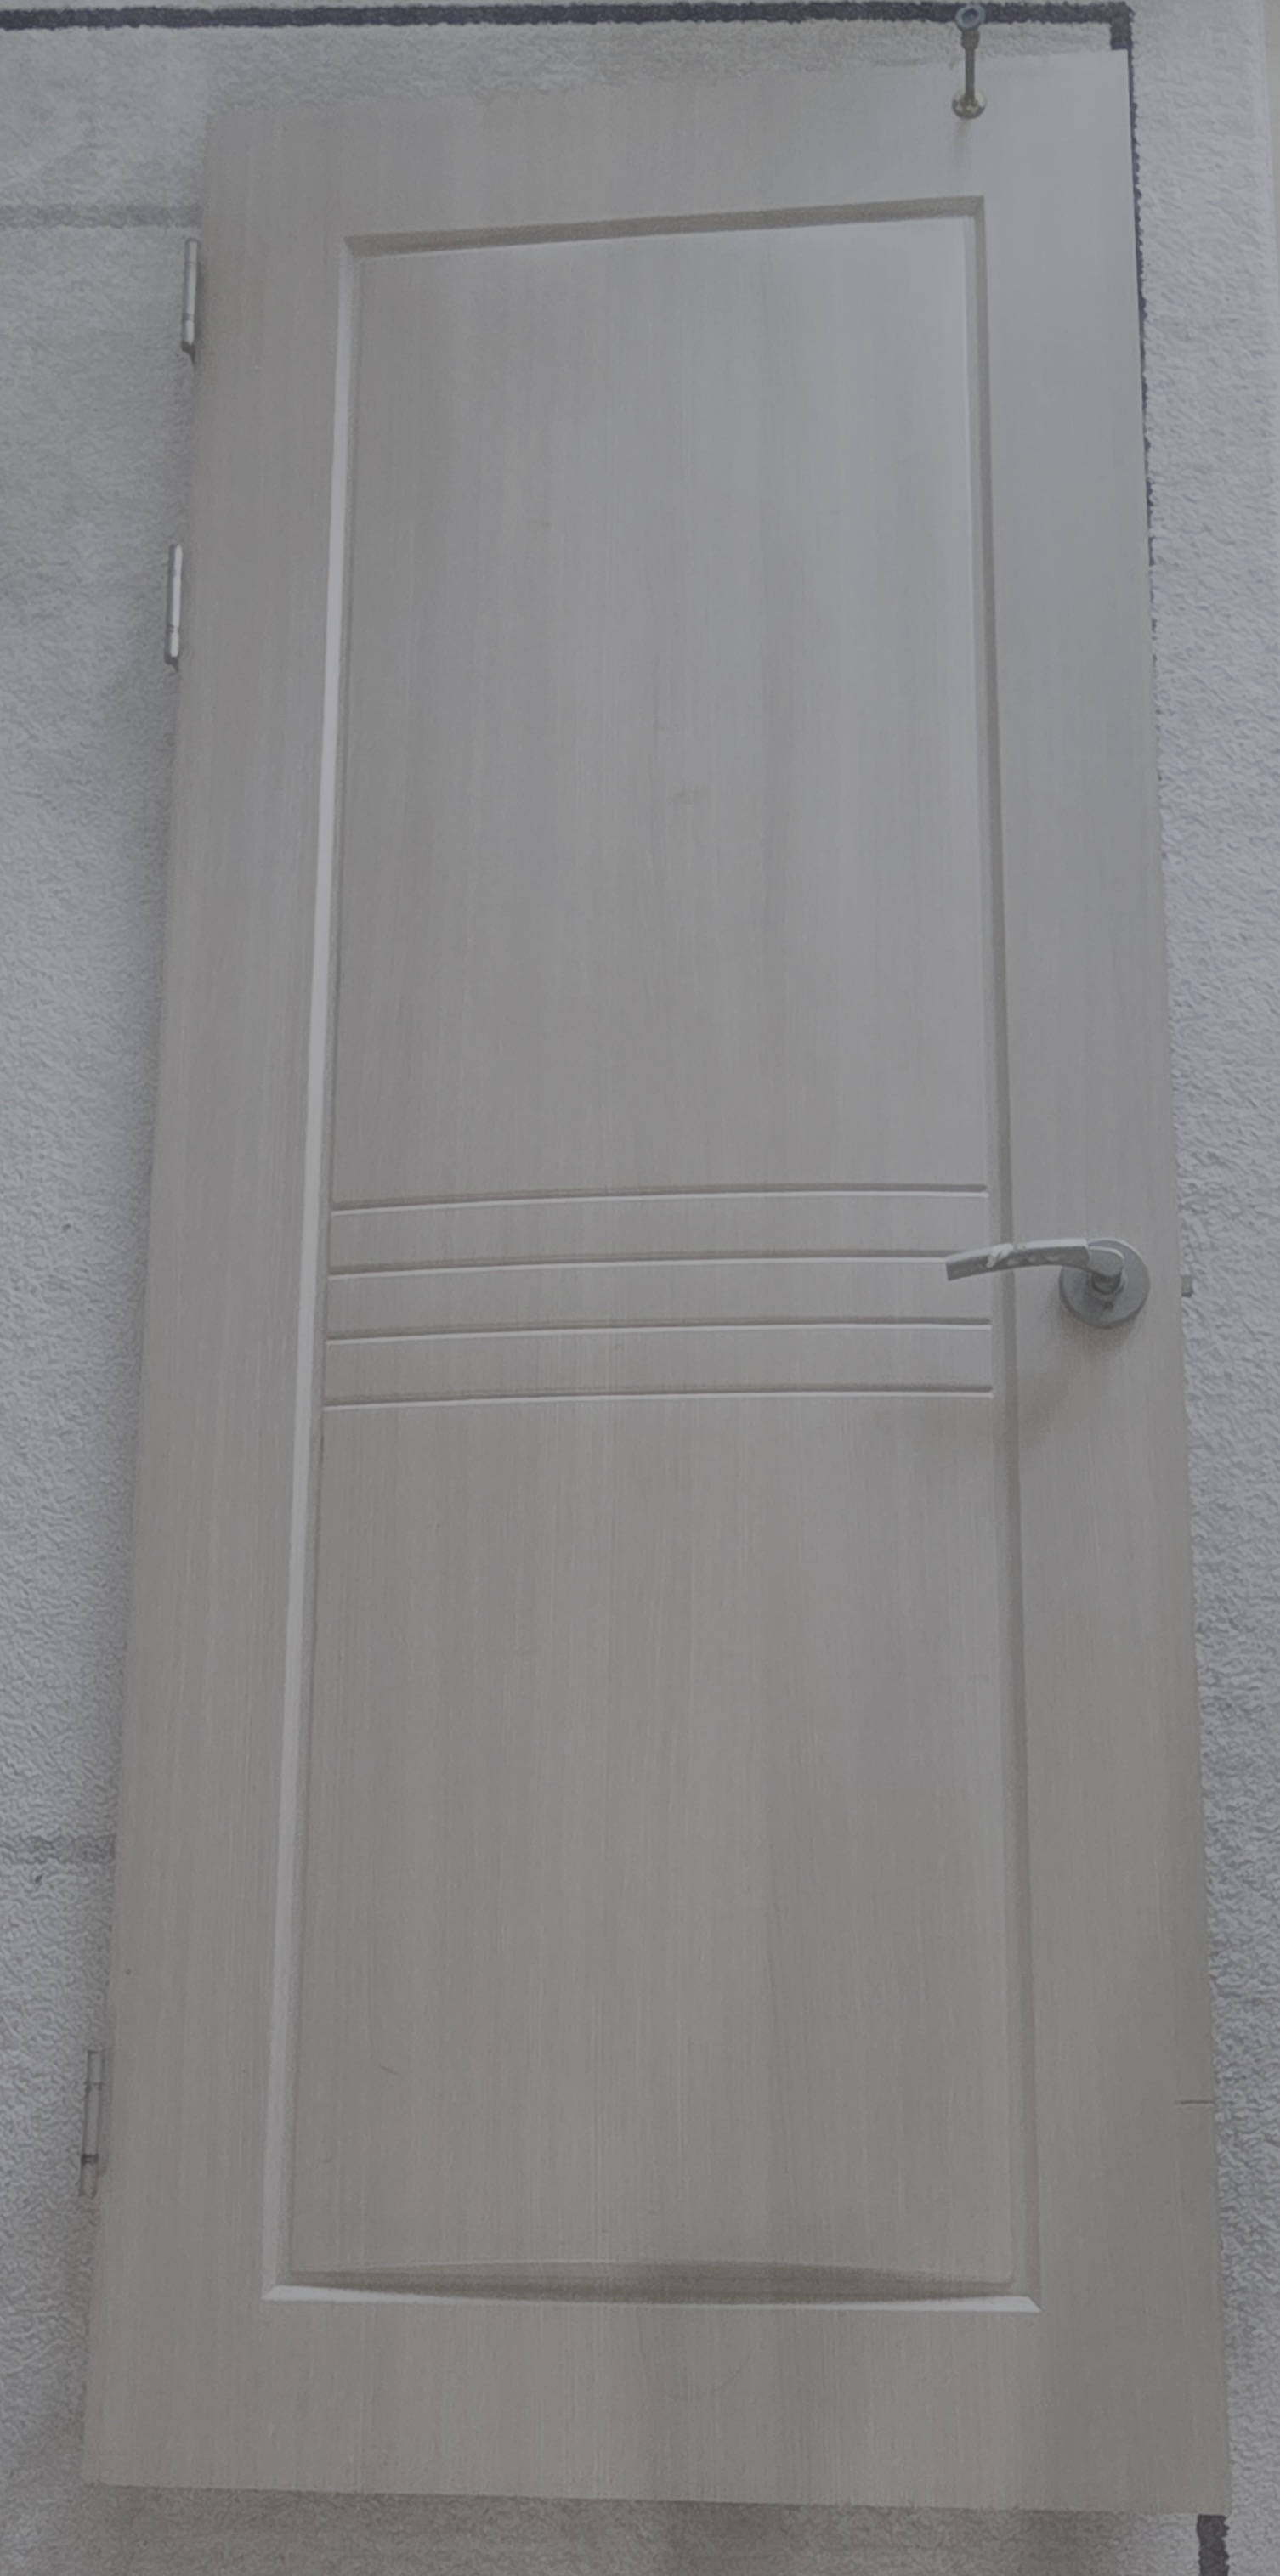
\includegraphics[width=\linewidth]{fig_door_removed.jpg}
\caption{The door detached for direct measurement of mass ($13.7$ kg) and dimensions.}
\label{fig:door_removed}
\end{minipage}\hfill
\begin{minipage}{0.48\textwidth}
\centering

\includegraphics[width=\linewidth]{fig_setup.jpg}
\caption{Experimental setup showing the smartphone (Samsung SM-S931N) attached to the door.}
\label{fig:setup}
\end{minipage}
\end{figure}

\begin{table}[h!]
\centering
\caption{Symbols and measured values for the door.}
\label{tab:variables}
\begin{tabular}{lll}
\toprule
\textbf{Symbol} & \textbf{Meaning} & \textbf{Value / unit} \\
\midrule
$m$ & mass of the door & $13.7$ kg \\
$w$ & width & $0.833$ m \\
$h$ & height & $2.031$ m \\
$r$ & hinge-to-phone distance & $0.759$ m \\
$\omega$ & angular velocity & rad/s \\
$\tau_f$ & frictional torque & N\,m \\
$a,b,c$ & dry, Stokes, Newton coefficients & N\,m, N\,m\,s, N\,m\,s$^2$ \\
$I=\tfrac13 mw^2$ & moment of inertia & $3.17$ kg\,m$^2$ \\
\bottomrule
\end{tabular}
\end{table}

% =========================================================================
\section{Step-by-Step Mathematical Derivations}
% =========================================================================
\subsection{Derivation of the Moment of Inertia}
 To analyze the rotational motion of a slammed door, the moment of inertia of the door about its hinge axis must be determined.\\
 The moment of inertia is defined as
 \begin{equation}\label{eq:start}
     I=\int r^2\,dm
 \end{equation}
 where $r$ is the perpendicular distance from the rotation axis to the mass element $dm$. The door is modeled as a rectangular solid with uniform mass density $\rho$, width $w$, height $h$, and thickness $d$. A Cartesian coordinate system is chosen such that the $z$-axis coincides with the hinge axis, the $x$-axis extends along the width of the door, and the $y$-axis extends through its thickness. The dimensions of the door are therefore
\begin{equation}
0 \le x \le w,\,0 \le y \le \ {d},\,0 \le z \le h.
\end{equation}
Since the door rotates about the $z$-axis, the perpendicular distance from a mass element to the rotation axis is
\begin{equation}
r^2=x^2+y^2.
\end{equation}
Substituting this expression into the definition of moment of inertia gives
\begin{equation}
I=\int (x^2+y^2)\,dm.
\end{equation}
Because the mass distribution is uniform, the infinitesimal mass element can be expressed as
\begin{equation}
dm=\rho\,dV,
\end{equation}
where
\begin{equation}
dV=dx\,dy\,dz.
\end{equation}
Thus,
\begin{equation}
dm=\rho\,dx\,dy\,dz.
\end{equation}
Substituting into the moment of inertia integral yields
\begin{equation}
I=\rho\int_0^h\int_{0}^{d}\int_0^w(x^2+y^2)\,dx\,dy\,dz.
\end{equation}
Separating the integral into two terms gives
\begin{equation}
I=\rho\int_0^{h}dz\int_{0}^{d}\int_0^w(x^2+y^2)\,dx\,dy\\
\end{equation}
\begin{equation}
I=\rho h\int_{0}^{d}(\frac{1}{3}w^3+wy^2)\,dy\\
\end{equation}
Since the thickness of a typical door is much smaller than its width $(d \ll w)$, the term containing $d^2$ is negligible compared with the term containing $w^2$. Therefore,
\begin{equation}
I=\frac{1}{3}\rho hwd(w^2+d^2)\approx\frac{1}{3}\rho hw^3d\\
\end{equation}
Using the relation
\begin{equation}
\rho=\frac{m}{dwh}
\end{equation}
the moment of inertia becomes
\begin{equation}
I \approx \frac{1}{3}mw^2.
\end{equation}

\subsection{Derivation of Frictional Torque Models}
In the original paper, the frictional torque acting on the rotating door is introduced as
\begin{equation}
\tau_f = a + b\omega + c\omega^2.
\end{equation}

However, the physical origin of each term is not discussed in detail. In this section, the three contributions are derived from fundamental physical principles.
\subsubsection{Dry friction Torque}
Dry friction originates from contact between the hinge surfaces. The friction force is given by
\begin{equation}
F_{\mathrm{dry}}=\mu N,
\end{equation}
which is approximately independent of velocity. Since torque is defined as
\begin{equation}
\tau=rF,
\end{equation}
the corresponding frictional torque is approximately constant,
\begin{equation}
\tau_{\mathrm{dry}}=a.
\end{equation}
\subsubsection{Stokes Friction Torque}
For motion through a fluid at low velocity, Stokes' law states that the resistive force is proportional to velocity,
\begin{equation}
F_{\mathrm{Stokes}}\propto v.
\end{equation}
For a rotating door, the linear velocity of a point at distance $r$ from the axis is
\begin{equation}
v=r\omega.
\end{equation}
Therefore,
\begin{equation}
\tau_{\mathrm{Stokes}}=rF_{\mathrm{Stokes}}
\propto r(r\omega),
\end{equation}
which leads to a torque proportional to angular velocity,
\begin{equation}
\tau_{\mathrm{Stokes}}=b\omega.
\end{equation}
\subsubsection{Newtonian Drag Torque}
At higher velocities, air resistance is described by the Newtonian drag equation
\begin{equation}
F_D=\frac12 C_D\rho A v^2.
\end{equation}
Since $v=r\omega$,
\begin{equation}
F_D\propto (r\omega)^2.
\end{equation}
The resulting torque is
\begin{equation}
\tau_D=rF_D
\propto r(r\omega)^2,
\end{equation}
which is proportional to the square of angular velocity,
\begin{equation}
\tau_D=c\omega^2.
\end{equation}

Combining all three contributions gives the general frictional torque model
\begin{equation}
\tau_f=a+b\omega+c\omega^2.
\end{equation}



\subsection{Derivation of the Equation of Motion}

After deriving the moment of inertia and the frictional torque model, the equation governing the rotational motion of the door can be obtained using Newton's second law for rotational systems.

For rotational motion about a fixed axis,

\begin{equation}
\sum\tau = I\alpha,
\end{equation}

where $I$ is the moment of inertia and $\alpha$ is the angular acceleration.

Since angular acceleration is defined as the time derivative of angular velocity,

\begin{equation}
\alpha=\frac{d\omega}{dt},
\end{equation}

Newton's second law becomes

\begin{equation}
\sum\tau = I\frac{d\omega}{dt}.
\end{equation}

The only torque considered in this model is the frictional torque opposing the motion of the door. Therefore,
\begin{equation}\label{eq:net_torque}
\sum\tau = -\tau_f.
\end{equation}
The negative sign appears because friction always acts opposite to the direction of rotation and therefore reduces the angular velocity.

Substituting the general frictional torque model,
\begin{equation}\label{eq:f_torque}
\tau_f=a+b\omega+c\omega^2,
\end{equation}
into Eq.~\eqref{eq:net_torque} gives
\begin{equation}\label{eq:ode}
-I\frac{d\omega}{dt}
=
a+b\omega+c\omega^2.
\end{equation}

This first-order nonlinear differential equation governs the rotational motion of the slammed door and serves as the starting point for all subsequent friction models analyzed in this study.



\subsection{Analytical Solutions of the Friction Models}
The original paper directly presents analytical solutions for the D, S, N, DS, DN, and SN models. While the derivation of the most general DSN model is already provided in the Appendix of the original paper, the intermediate mathematical steps leading to the remaining analytical solutions are omitted. Therefore, this section derives the D, S, N, DS, DN, and SN models in detail, starting from the governing differential equation obtained in the previous section.
\subsubsection{Dry Friction Model (D)}
For the dry friction model, only the constant friction term is considered. The governing equation becomes
\begin{equation}
-I\frac{d\omega}{dt}=a.
\end{equation}
Rearranging and integrating,
\begin{equation}
\int d\omega=-\frac{a}{I}\int dt.
\end{equation}
Applying the initial condition $\omega(0)=\omega_0$, the solution is
\begin{equation}
\boxed{
\omega_D(t)=\omega_0-\frac{a}{I}t}.
\end{equation}
This model predicts a linear decrease in angular velocity.
\subsubsection{Stokes Friction Model (S)}
For the Stokes friction model,
\begin{equation}
-I\frac{d\omega}{dt}=b\omega.
\end{equation}
Separating variables,
\begin{equation}
\frac{d\omega}{\omega}=-\frac{b}{I}dt.
\end{equation}
Integrating both sides and applying the initial condition $\omega(0)=\omega_0$ gives
\begin{equation}
\boxed{
\omega_S(t)=\omega_0e^{-bt/I}
}.
\end{equation}
This solution represents exponential decay.
\subsubsection{Newtonian Drag Model (N)}
For the Newtonian drag model,
\begin{equation}
-I\frac{d\omega}{dt}=c\omega^2.
\end{equation}
Separating variables,
\begin{equation}
\frac{d\omega}{\omega^2}=-\frac{c}{I}dt.
\end{equation}
Integrating both sides and applying the initial condition $\omega(0)=\omega_0$ gives
\begin{equation}
\boxed{
\omega_N(t)=\frac{\omega_0}{1+\dfrac{c\omega_0}{I}t}
}.
\end{equation}  
Unlike the D and S models, the Newtonian model predicts an inverse-time decay of angular velocity.



\subsubsection{Dry and Stokes Friction Model (DS)}

For the DS model, the Newtonian drag term is neglected $(c=0)$. The governing equation becomes

\begin{equation}
-I\frac{d\omega}{dt}=a+b\omega.
\end{equation}

Separating variables,

\begin{equation}
\frac{d\omega}{a+b\omega}
=
-\frac{1}{I}dt.
\end{equation}

Integrating both sides and applying the initial condition $\omega(0)=\omega_0$ yields

\begin{equation}
\boxed{
\omega_{DS}(t)
=
\left(\omega_0+\frac{a}{b}\right)
\exp\left(-\frac{bt}{I}\right)
-\frac{a}{b}
}.
\end{equation}

\subsubsection{Dry and Newtonian Drag Model (DN)}

For the DN model, the Stokes friction term is neglected $(b=0)$. The governing equation becomes

\begin{equation}
-I\frac{d\omega}{dt}
=
a+c\omega^2.
\end{equation}

Separating variables,

\begin{equation}
\frac{d\omega}{a+c\omega^2}
=
-\frac{1}{I}dt.
\end{equation}

Using the standard integral

\begin{equation}
\int\frac{dx}{a+cx^2}
=
\frac{1}{\sqrt{ac}}
\tan^{-1}
\left(
\sqrt{\frac{c}{a}}x
\right),
\end{equation}

and applying the initial condition $\omega(0)=\omega_0$, we obtain

\begin{equation}
\boxed{
\omega_{DN}(t)
=
\frac{
\omega_0
-
\sqrt{\frac{a}{c}}
\tan\!\left(\frac{\sqrt{ac}}{I}t\right)
}
{
1+
\omega_0
\sqrt{\frac{c}{a}}
\tan\!\left(\frac{\sqrt{ac}}{I}t\right)
}
}.
\end{equation}

\subsubsection{Stokes and Newtonian Drag Model (SN)}

For the SN model, the dry friction term is neglected $(a=0)$. The governing equation becomes

\begin{equation}
-I\frac{d\omega}{dt}
=
b\omega+c\omega^2.
\end{equation}

Separating variables,

\begin{equation}
\frac{d\omega}
{\omega(b+c\omega)}
=
-\frac{1}{I}dt.
\end{equation}

Using partial fraction decomposition and applying the initial condition $\omega(0)=\omega_0$, the solution becomes

\begin{equation}
\boxed{
\omega_{SN}(t)
=
\frac{
-b\omega_0
}
{
c\omega_0
-
(\omega_0 c+b)
\exp\!\left(\frac{bt}{I}\right)
}
}.
\end{equation}

% =========================================================================
\section{Physical Approximations and Limiting Cases}
% =========================================================================
It is useful to ask in advance how distinguishable these solutions are. Expanding each for
small $t$,
\begin{equation}
\omega(t)\approx\omega_0-\bigl(A+B\omega_0+C\omega_0^2\bigr)\,t+\mathcal{O}(t^2),
\end{equation}
so that to first order every model reduces to a straight line with the same initial slope.
The curvature that distinguishes the dry, Stokes, and Newtonian cases appears only after
$\omega$ has changed appreciably. A door slammed hard reaches the frame within a fraction of
a second and loses little of its angular velocity beforehand, so its free-rotation record is
short and nearly linear, and such a record cannot by itself separate the models.

\begin{physicsinsight}
A nearly linear $\omega(t)$ suggests a constant torque, and hence dry friction. Klein et
al.\ caution against this inference, noting that over a limited range the data ``look quite
linear'' even though this appearance does not constitute evidence for the dry model. The
resolution is to set the fit quality aside and ask whether the fitted coefficient is
physically reasonable, the approach taken in Section~5.
\end{physicsinsight}

The two drag laws also correspond to different flow regimes. Stokes drag applies at low
Reynolds number and Newtonian drag at high Reynolds number. A door moving through air at of
order $1\,\mathrm{rad/s}$ lies well within the high-Reynolds regime, which already indicates
which term is expected to dominate physically.

% =========================================================================
\section{Computational and Experimental Verification}
% =========================================================================
\subsection{Measurement}
A smartphone (Samsung SM-S931N) was attached to the door, and the gyroscope rotation rate
was recorded with the Phyphox application at approximately $460$~Hz. Two trials were taken, a
hard (fast) slam and a gentle (slow) one, corresponding to a large and a small initial spin.
Each record consists of an initial push, a free-rotation phase governed only by friction,
and a sharp spike as the door meets the frame. Only the free-rotation phase is analysed. The
short interval immediately before impact, in which the deceleration increases as air is
compressed against the frame, is excluded, because no term in Eq.~\eqref{eq:ode} can produce
a growing $|d\omega/dt|$ and the effect is therefore physically distinct.
Figure~\ref{fig:overview} shows the complete traces with the analysed windows shaded.

\begin{figure}[h!]
\centering
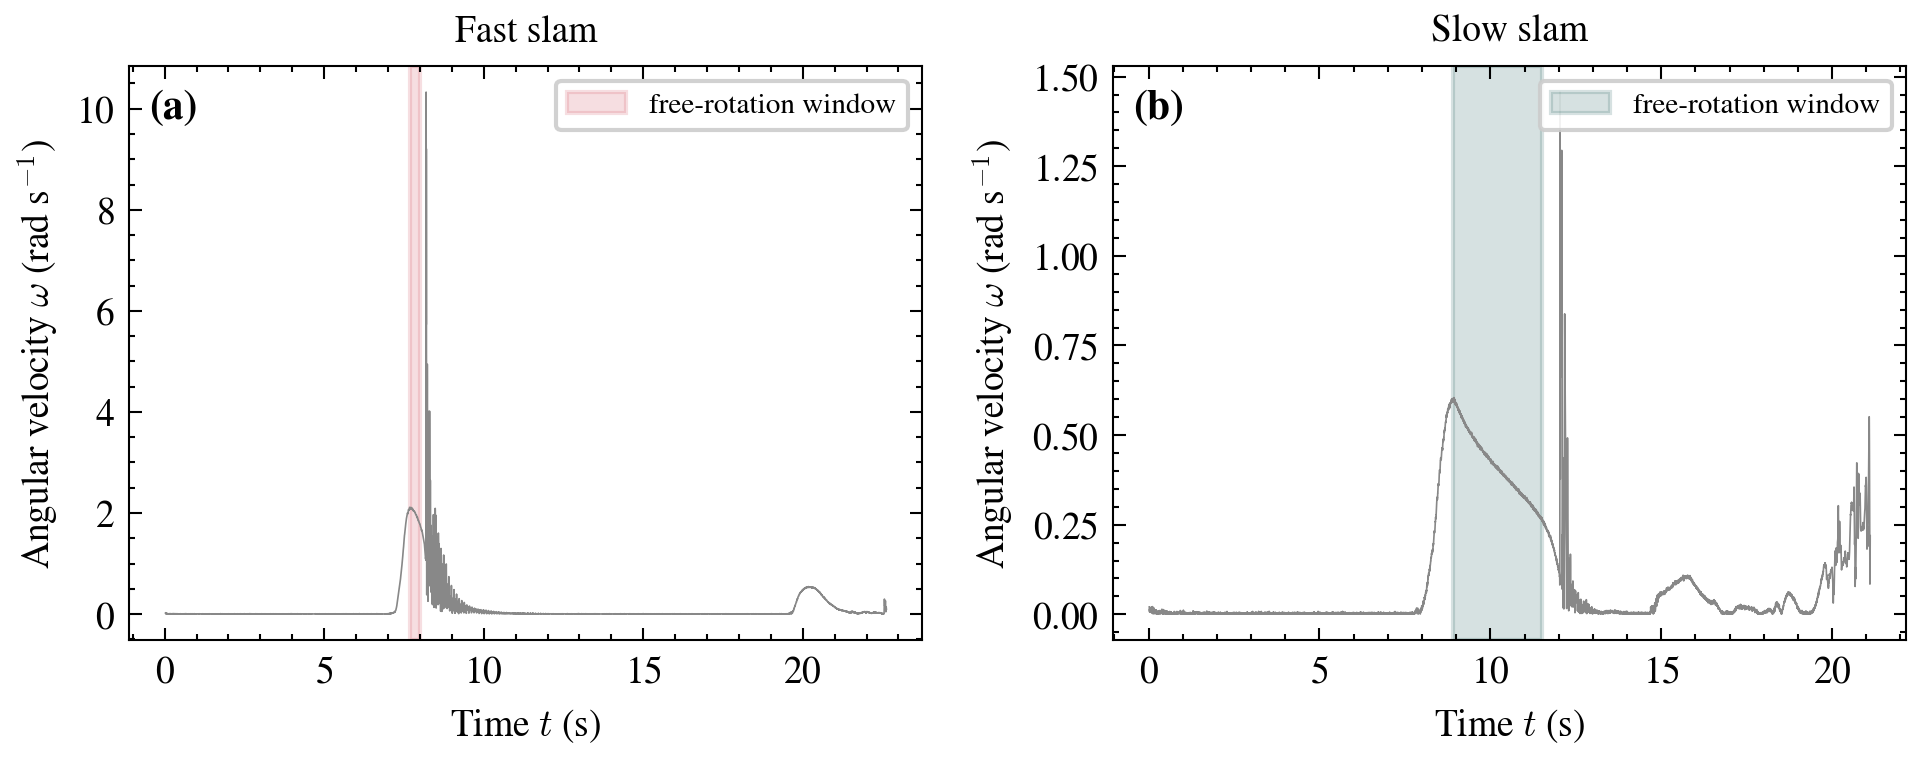
\includegraphics[width=\linewidth]{fig1_overview.png}
\caption{Gyroscope traces for the two slams, with the free-rotation windows shaded. The
sharp spikes mark the impact with the frame and are excluded from the fits.}
\label{fig:overview}
\end{figure}

\subsection{Fits to the Six Models}
Each model was fitted with \texttt{scipy.optimize.curve\_fit}. The resulting parameters and
fit quality are given in Tables~\ref{tab:fits_fast} and~\ref{tab:fits_slow}, and the fitted
curves are shown in Fig.~\ref{fig:fits}. In the fast slam the angular velocity decreases only
from $2.08$ to $1.79~\mathrm{rad/s}$, that is, to $0.86\,\omega_0$, and as anticipated in
Section~3 all six models fit almost equally well, with $R^2$ between $0.92$ and $0.94$. The
slow slam spans a wider range, from $0.60$ to $0.27~\mathrm{rad/s}$, and the differences
between the models become apparent. A nested $F$-test comparing the dry model with the
dry-plus-Newton model gives $F\approx4\times10^{3}$ ($p<0.001$), so that a purely linear law
is statistically inadequate and the data require curvature.

% --- Fast slam (window 7.69-8.0 s, n=144) ---
\begin{table}[h]\centering
\caption{Fitting parameters and goodness-of-fit --- fast slam.}
\label{tab:fits_fast}
\begin{tabular}{lcccccc}
\toprule
Model & $a/I$ & $b/I$ & $c/I$ & $R^2$ & SSE & $\Delta$AIC \\
\midrule
\textbf{D} & 1.088 & -- & -- & 0.9441 & 0.08098 & 0.0 \\
S & -- & 0.5432 & -- & 0.9343 & 0.0952 & 23.3 \\
N & -- & -- & 0.2706 & 0.9238 & 0.1104 & 44.7 \\
DS & 1.088 & 1.923e-07 & -- & 0.9441 & 0.08098 & 2.0 \\
DN & 1.088 & -- & 4.58e-18 & 0.9441 & 0.08098 & 2.0 \\
SN & -- & 0.5432 & 1.78e-20 & 0.9343 & 0.0952 & 25.3 \\
\bottomrule
\end{tabular}
\end{table}

% --- Slow slam (window 8.9-11.5 s, n=1206) ---
\begin{table}[h]\centering
\caption{Fitting parameters and goodness-of-fit --- slow slam.}
\label{tab:fits_slow}
\begin{tabular}{lcccccc}
\toprule
Model & $a/I$ & $b/I$ & $c/I$ & $R^2$ & SSE & $\Delta$AIC \\
\midrule
D & 0.1203 & -- & -- & 0.9879 & 0.12 & 1785.3 \\
S & -- & 0.2911 & -- & 0.9967 & 0.03321 & 236.5 \\
N & -- & -- & 0.6752 & 0.9896 & 0.103 & 1601.9 \\
DS & 0.0001393 & 0.2908 & -- & 0.9967 & 0.03321 & 238.5 \\
\textbf{DN} & 0.05793 & -- & 0.3556 & 0.9973 & 0.02725 & 0.0 \\
SN & -- & 0.2699 & 0.0495 & 0.9967 & 0.03277 & 222.4 \\
\bottomrule
\end{tabular}
\end{table}


\begin{figure}[h!]
\centering
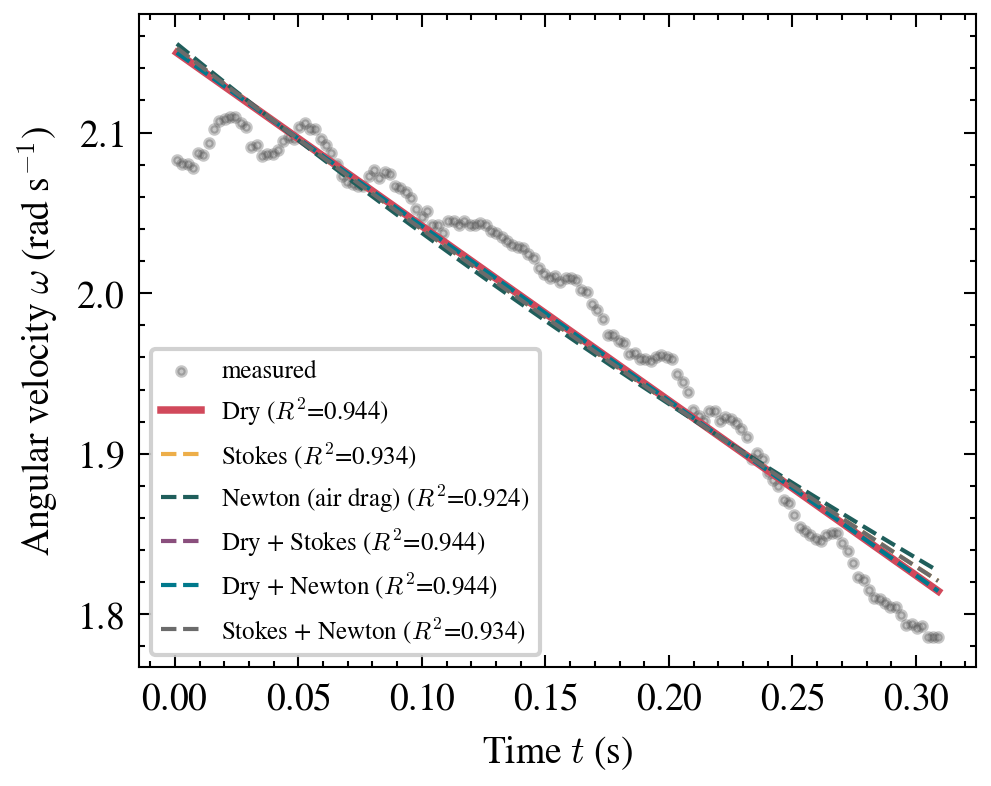
\includegraphics[width=0.49\linewidth]{fig_fit_fast.png}\hfill
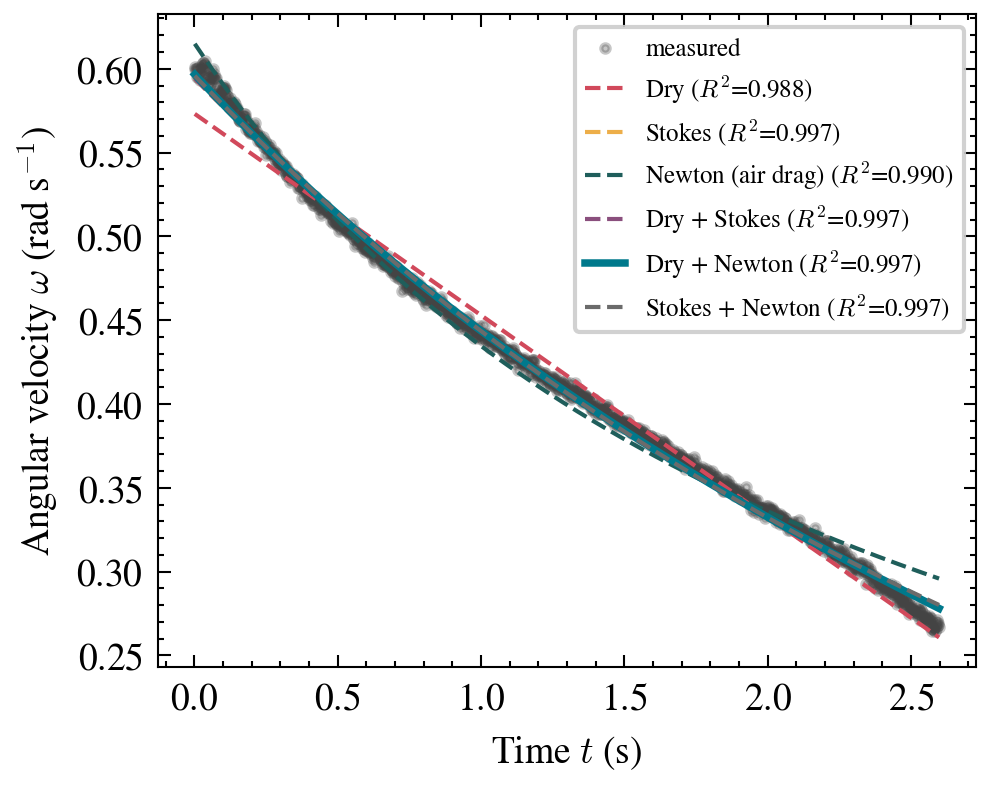
\includegraphics[width=0.49\linewidth]{fig_fit_slow.png}
\caption{Six-model fits to the free-rotation phase of the fast (left) and slow (right)
slams. In the slow case the straight dry-friction line clearly misses the curvature of the
data.}
\label{fig:fits}
\end{figure}

The fit quality is quantitatively compared in Fig.~\ref{fig:gof}, showing the $R^2$ values and the Information Criterion (AIC). While $R^2$ is high for all models, the $\Delta$AIC clearly penalizes models that fail to capture the curvature, especially in the slow slam case.

\begin{figure}[h!]
\centering
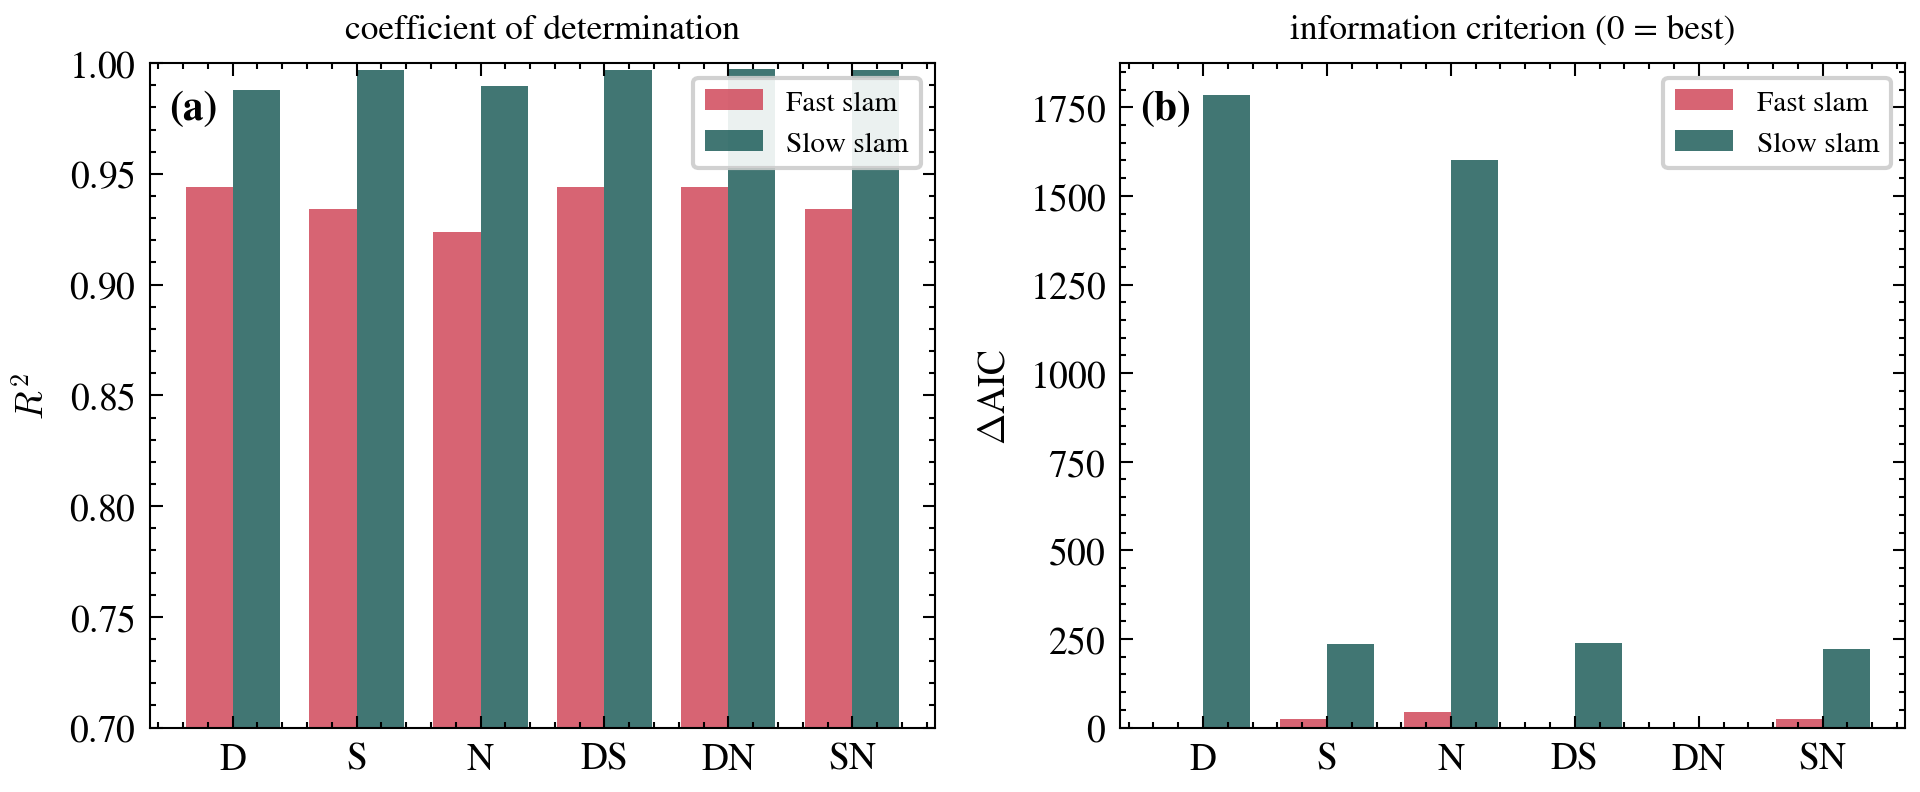
\includegraphics[width=\linewidth]{fig3_gof.png}
\caption{Comparison of fit quality for all six models across the two slams: (a) coefficient of determination $R^2$, and (b) relative Information Criterion $\Delta$AIC (lower is better).}
\label{fig:gof}
\end{figure}

\subsection{Numerical Check of the Analytical Solutions}
To confirm the closed-form expressions of Section~2, Eq.~\eqref{eq:ode} was integrated
directly with \texttt{scipy.integrate.solve\_ivp} (RK45) using the fitted coefficients, and
the result was compared with the analytic curve (Fig.~\ref{fig:sim}). The two agree to about
$10^{-8}~\mathrm{rad/s}$, which is at the level of numerical round-off and confirms the
derivations. The same routine also applies to the general model, for which no simple closed
form is available.

\begin{figure}[h!]
\centering
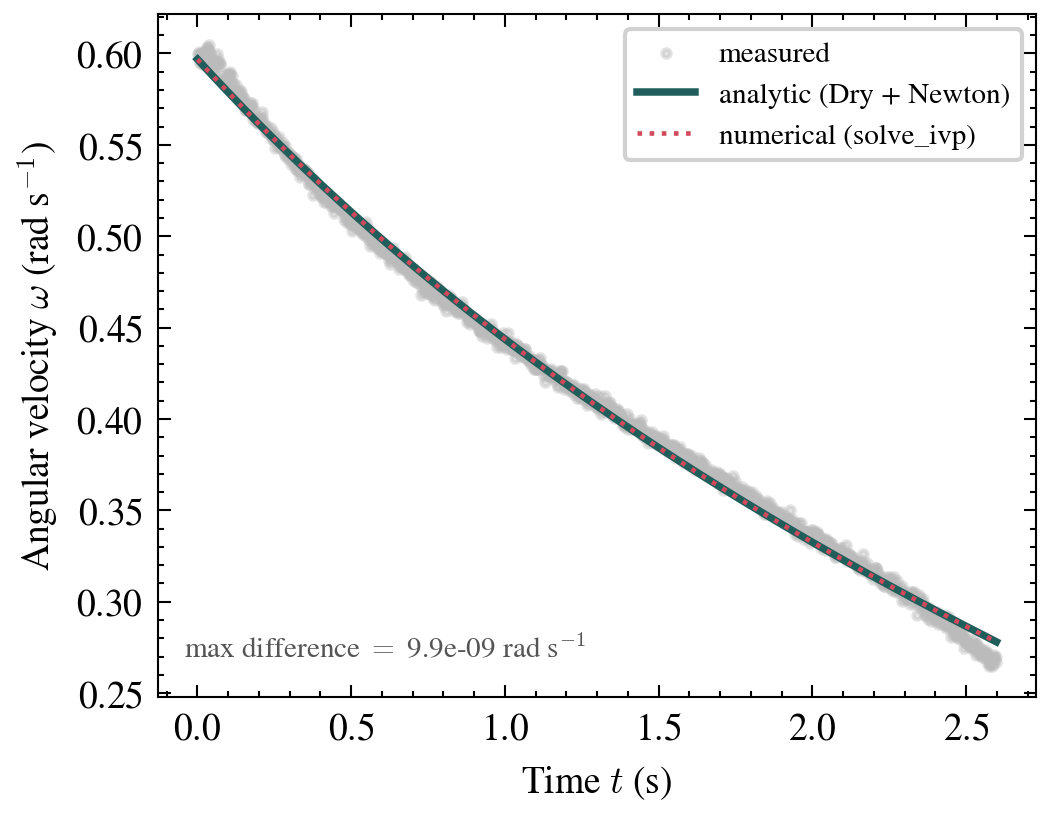
\includegraphics[width=0.85\linewidth]{fig4_simulation.png}
\caption{Analytic solution versus direct numerical integration for the slow slam. The curves
are indistinguishable (maximum difference $\sim10^{-8}$~rad/s).}
\label{fig:sim}
\end{figure}

\subsection{Comparative Analysis of Simulation Models}
To further investigate the qualitative differences between the friction mechanisms, all six models were simulated over a longer duration until the door comes to a complete rest. Using the numerical integration framework established in Section 4.3, we compare the velocity decay profiles for the Dry, Stokes, Newtonian, and combined models.
A visual representation of the door motion governed by the full DSN model is shown in Fig.~\ref{fig:door_strip}, illustrating how the door's angular position changes over time as it approaches the frame.
As shown in Fig.~\ref{fig:sim_models}, the models diverge significantly as the angular velocity decreases. The dry friction model predicts a linear decrease and a finite stopping time, while the Stokes and Newtonian models exhibit characteristic exponential and inverse-time asymptotic behaviors, respectively. This comprehensive simulation, conducted by Seong, confirms that while models may appear similar in the high-velocity regime of a fast slam, their long-term dynamics are governed by the specific velocity dependence of the frictional torque.

\begin{figure}[h!]
\centering
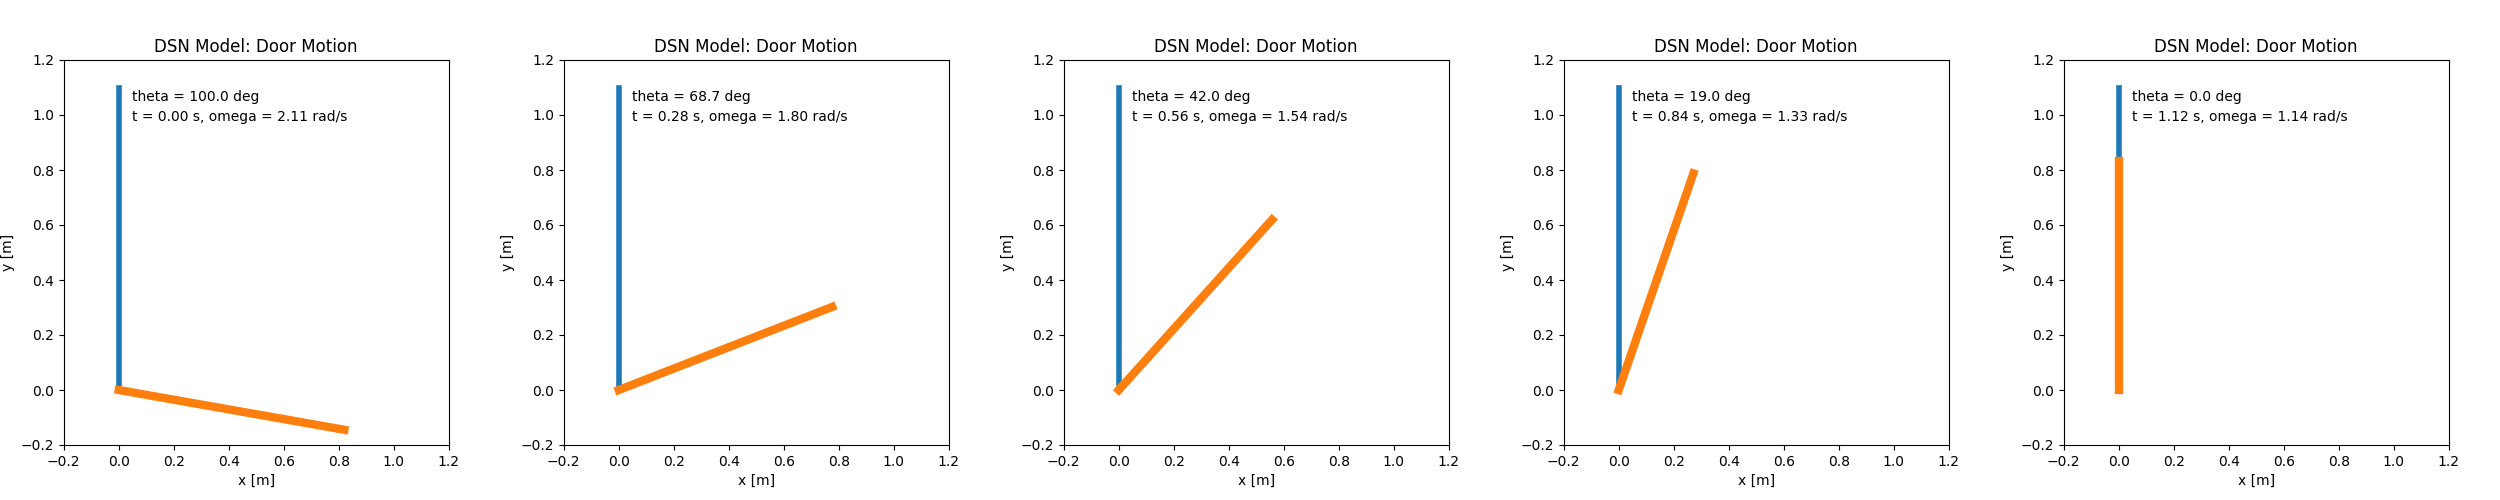
\includegraphics[width=\linewidth]{fig7_door_strip.png}
\caption{Stroboscopic visualization of the door motion simulated using the full DSN friction model, showing the angular displacement from $100^\circ$ to impact.}
\label{fig:door_strip}
\end{figure}

\begin{figure}[h!]
\centering
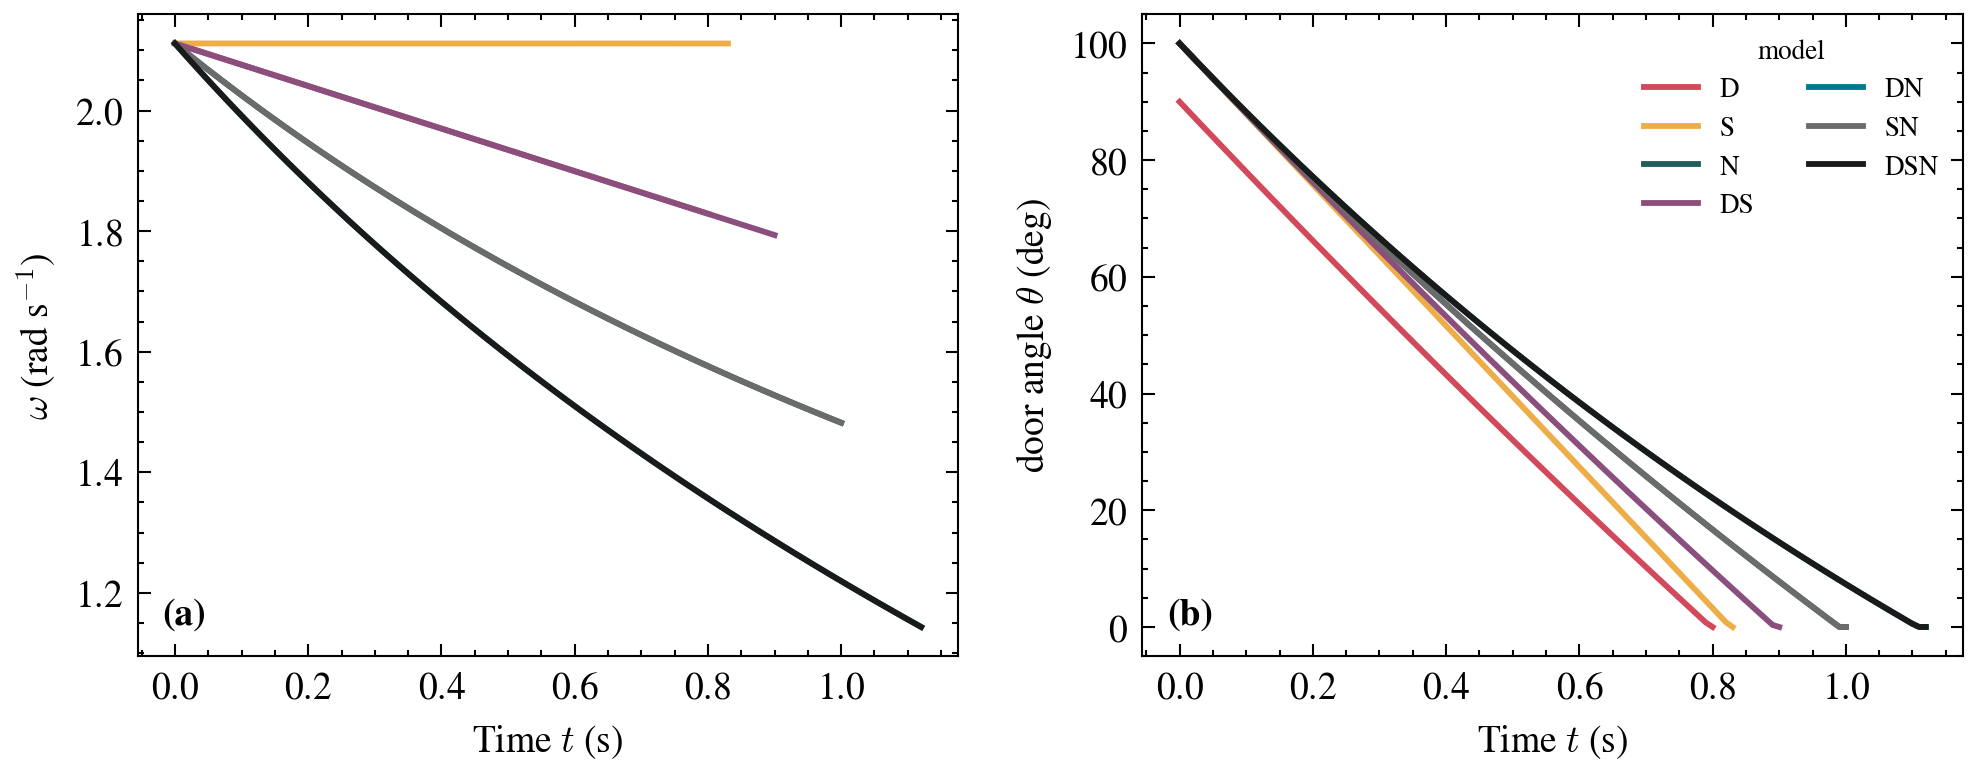
\includegraphics[width=\linewidth]{fig6_sim_models.png}
\caption{Comparison of the six friction models over an extended simulation time. The distinct decay characteristics of constant (dry), linear (Stokes), and quadratic (Newtonian) terms are clearly visible.}
\label{fig:sim_models}
\end{figure}

% =========================================================================
\section{Critical Analysis and Commentary}
% =========================================================================
Because goodness of fit alone cannot select among the models, each fitted coefficient is
compared with an order-of-magnitude estimate obtained from first principles, following the
original paper. For dry friction $a/I=3\mu g/w$, for Stokes drag $b/I\lesssim 18\pi\eta w/m$,
and for Newtonian drag $c/I\lesssim\tfrac32 C_D\rho A w/m$, with
$\eta=1.7\times10^{-5}~\mathrm{Pa\,s}$, $\rho=1.3~\mathrm{kg/m^3}$, and $C_D=1.5$. The
comparison is summarised in Table~\ref{tab:validity} and Fig.~\ref{fig:validity}.

\begin{table}[h]\centering
\caption{Order-of-magnitude validity of the fitted friction coefficients (cf. Klein et al.).}
\label{tab:validity}
\begin{tabular}{llll}
\toprule
Coefficient & Fitted (fast / slow) & Theoretical estimate & Verdict \\
\midrule
$a/I$ (Dry) & 1.088 / 0.120 & $3\mu g/w$, $\mu$=0.031/0.0034 & Rejected ($\mu$ 9$\times$ inconsistent) \\
$b/I$ (Stokes) & 0.543 / 0.291 & $\sim 6\times10^{-5}$ & Rejected ($10^3$--$10^4\times$ too large) \\
$c/I$ (Newton) & 0.271 / 0.675 & $\lesssim 0.30$ & \textbf{Accepted (same order)} \\
\bottomrule
\end{tabular}
\end{table}


\begin{figure}[h!]
\centering
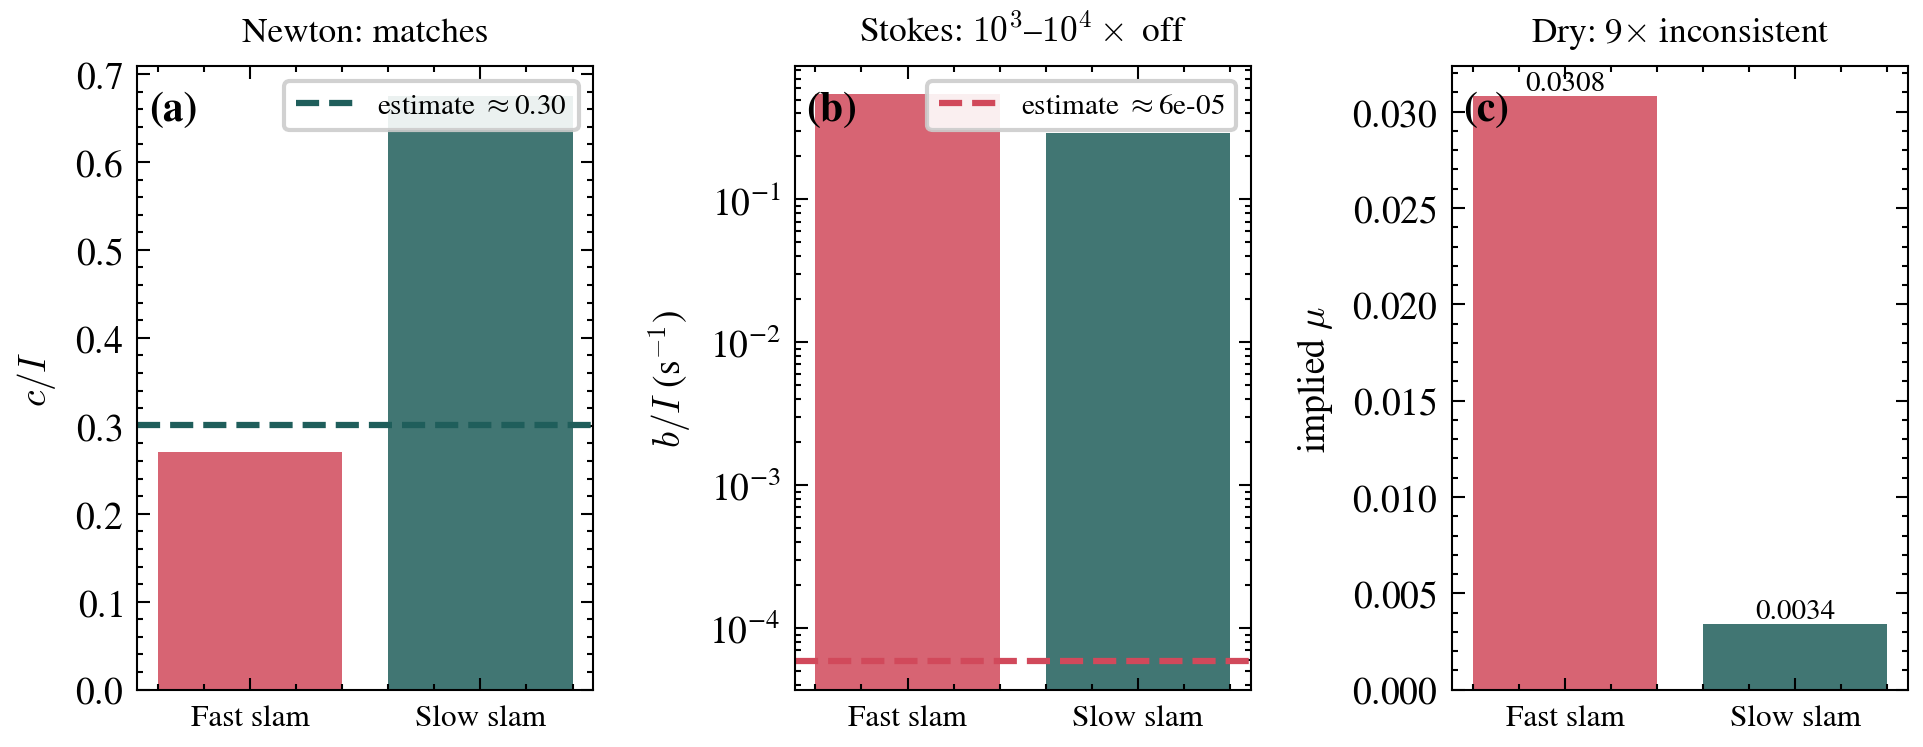
\includegraphics[width=\linewidth]{fig5_validity.png}
\caption{Fitted coefficients against their physical estimates. The Newtonian $c/I$ lands on
the predicted value; the Stokes $b/I$ overshoots by three to four orders of magnitude; and
the dry-friction coefficient implies two incompatible values of $\mu$.}
\label{fig:validity}
\end{figure}

The fitted Stokes coefficient is of order $0.3$ to $0.6~\mathrm{s^{-1}}$, roughly $10^{3}$
to $10^{4}$ times the estimate of $6\times10^{-5}~\mathrm{s^{-1}}$, so that Stokes drag is
far too weak to account for the observed deceleration. The dry-friction model appears
adequate until the implied sliding coefficient is examined. It is $\mu\approx0.031$ for the
fast slam and $\mu\approx0.0034$ for the slow one, a factor of nine apart. Since $\mu$ is a
material constant and cannot depend on the initial spin, the dry model is internally
inconsistent; Klein et al.\ rejected it on the analogous ground that the implied torque was
unreasonably large. The Newtonian coefficient is the only one consistent with its estimate.
The fitted values $c/I=0.27$ (fast) and $0.68$ (slow) are of the same order as the predicted
$0.30$, and the increase of $c/I$ at lower spin reproduces the trend reported in the
original paper, which attributed it to the Reynolds-number dependence of $C_D$.

The limitations of the measurement should also be noted. The fast slam is too short to
discriminate the models on its own; the same limitation of the slammed-door method is
reported in the original paper, where $\omega$ decreases only to about $0.75\,\omega_0$
before impact. In this shorter and noisier window the unconstrained fit even favours the
simplest (dry) model slightly, which is the situation described in Section~3 and is resolved
by the physical-validity test. Klein et al.\ avoided the difficulty with a separate, longer
laboratory experiment on a light plate. The natural extension of the present work is to
repeat the measurement with the door released from a wider angle at higher spin, so that it
decelerates over a longer arc without striking the frame. Further sources of uncertainty
include gyroscope noise, which appears as the lower $R^2$ of the fast window, the
uncertainty in $r$, and the thin-plate approximation for $I$.

% =========================================================================
\section{Conclusion}
% =========================================================================
A real door was measured with a smartphone gyroscope, the friction models of Klein et al.\
were reconstructed with their intermediate steps supplied, and the analytic solutions were
verified by direct numerical integration. Of the six models, the Stokes and dry-friction
terms are excluded on physical grounds, the former by a discrepancy of three to four orders
of magnitude in its coefficient and the latter by a coefficient that does not remain
constant between trials, leaving the quadratic Newtonian air-drag term as the only
physically consistent description. This agrees with the conclusion of the original paper.
Beyond the specific result, the project illustrates a general methodological point, that
agreement with the data is not sufficient to establish a model and that the fitted
parameters must be confronted with independent physical reasoning.

\begin{thebibliography}{9}
\bibitem{klein2017} P.~Klein, A.~M\"uller, S.~Gr\"ober, A.~Molz, and J.~Kuhn,
``Rotational and frictional dynamics of the slamming of a door,''
\textit{American Journal of Physics} \textbf{85}(1), 30--37 (2017).
\bibitem{repo} Team solvE, \textit{physics-door-slam}, analysis code and data,
\url{https://github.com/eeuunn/physics-door-slam}.
\end{thebibliography}
\end{document}
